% !TEX root = SegwayDoku.tex


% tragt hier eure Unterdokumente in der Reihenfolge ein,
% in der sie im Gesamtdokument auftauchen sollen

% !TEX root = SegwayDoku.tex
\renewcommand{\autoren}{Stephan Morongowski}
\newpage
\section{Definition eines roboterfesten Koordinatensystems}

\begin{figure}[h]  % [h] bedeutet, dass das Bild genau an dieser Stelle im Text erscheint
\centering\includegraphics[width=0.6\textwidth]{images/FahrzeugKSys_mod.png}
\caption[Roboterkoordinatensystem]{Roboterkoordinatensystem \newline (Quelle: \cite{roboterKS_Bild})}
\label{robotKSys}
\end{figure}

Zur einheitlichen Bezeichnung wurde das roboterfeste Koordinatensystem (im Folgenden mit KS bezeichnet) wie in Abbildung \ref{robotKSys} zu sehen, ähnlich ISO 88551 festgelegt. Entgegen der häufig anzutreffenden Bezeichnungen der Winkel um die jeweiligen Koordinatenachsen werden im Folgenden die Winkel um
\begin{itemize}
    \item die x-Achse mit \(\alpha\)
    \item die y-Achse mit \(\beta\)
    \item die z-Achse mit \(\gamma\)
\end{itemize}
bezeichnet. \\
Der Ursprung des KS liegt auf der Radachse mittig zwischen den beiden Rädern.\\
Das KS ist ein rechtshändiges KS.\\\\
Die Verdrehung der jeweiligen Räder wird mit \(\varphi_l\) bzw. \(\varphi_r\) bezeichnet. Dabei bezeichnet \(l\) das in positive x-Richtung blickend links liegende Rad und \(r\) das in positive x-Richtung blickend rechts liegende Rad.

% !TEX root = ../SegwayDoku.tex
\renewcommand{\autoren}{Severin Schendel	}
%\newpage
\subsection{Vergleich der Antriebsarten}
\subsubsection{Bürstenloser Gleichstrommotor}

\begin{quote}
"Bürstenlose Gleichstrommotoren, kurz BLDC („Brushless DC-Motoren), sind -  entgegen ihrer Bezeichnung - Drehstrom-Synchronmaschinen: Der Läufer folgt einem magnetischen Drehfeld, die Bewegung ist synchron zur Wechselspannung, die an die Wicklungen angelegt wird. Dieser Motortyp wird häufig als „Bürstenloser Gleichstrommotor“ bezeichnet, da er in vielen Applikationen bürstenbehaftete Gleichstrommotoren („brushed DC“, Kommutatormotoren) ersetzt. Bei einem bürstenbehafteten Gleichstrommotor wird eine Gleichspannung angelegt, die durch einen mechanischen Wechselrichter im Motor - die Bürsten - einen drehzahlunabhängigen Wechselstrom erzeugt.

Zusammen mit einer elektronischen Ansteuerung, die die Funktion der Bürsten übernimmt und aus den eingespeisten Gleichstrom in Wechselstrom umwandelt, entspricht der BLDC-Motor im Verhalten einem bürstenbehafteten Gleichstrommotor ohne die in der Lebensdauer begrenzten Bürsten.  BLDC-Motoren werden deshalb auch als EC („electronically commutated“)-Motoren bezeichnet, um sie von mechanisch kommutierten bürstenbehafteten Motoren abzugrenzen."
\end{quote}
(Quelle: \cite{BLDCNanotec})
\begin{figure}[h]  % [h] bedeutet, dass das Bild genau an dieser Stelle im Text erscheint
\centering\includegraphics[width=0.7\textwidth]{images/BLDC_Prinzipschaltung}
\caption{BLDC Prinzipschaltung, V1-V6 MOSFETS \newline (Quelle: \cite{PrinzipBLDC})}
\label{PrinzipBLDC}
\end{figure}
\newpage

% !TEX root = BLDC_Schrittmotoren_Technologie.tex
\renewcommand{\autoren}{Severin Schendel	}
\newpage

\subsection{Schrittmotoren}
\subsubsection{Allgemeines}
Schrittmotoren sind eine spezielle Bauform der Synchronmaschine, bei denen der Rotor als Permanentmagnet ausgeführt ist, während der Stator aus einem Spulenpaket besteht. Im Unterschied zum Synchronmotor hat der Schrittmotor eine große Zahl an Polpaaren. Die Drehung des Rotors kommt dadurch zustande, dass das elektromagnetische Feld der Stators Sprungweiße geschalten wird und sich um einen Schrittwinkel bewegt.

Zum Betrieb des Motors wird eine spezielle Ansteuereinheit(Treiber) benötigt.

\subsubsection{Arten des Schrittmotors}

Es gibt drei Grundtypen des Schrittmotors.

\begin{itemize}
	\item Reluktanzschrittmotor (VR)
	\item Permanenterregter Schrittmotor(PM)
	\item Hybridschittmotor(HY)
\end{itemize}

\begin{figure}[h]  % [h] bedeutet, dass das Bild genau an dieser Stelle im Text erscheint
\centering\includegraphics[width=1.0\textwidth]{images/Schrittmotortypen.png}
\caption{Schrittmotortypen \newline (Quelle: \cite{roboterKS_Bild})}
\label{robotKSys}
\end{figure}

Für unseren Anwendungsfall kommt nur der Hybridschrittmotor in Frage, aufgrund des Haltemomentes von 03 bis 1000 cNm und des kleinen Schrittwinkel von $0,36^\circ$.

\subsubsection*{Hybridschrittmotor}
Der Hybridschrittmotor vereint die positiven Eigenschaften des Reluktanzschrittmotor und des Permanenterregten Schrittmotor. Sein Rotor besteht aus einem axialen Permanentmagneten, an dessen Enden gezahnte Kappen befestigt sind. Beide sind um eine halbe Zahnbreite gegeneinander versetzt, so das sich Nord- und Südpole abwechseln.

\subsubsection{Arten der Ansteuerung}
Es gibt drei Möglichkeiten Schrittmotoren anzusteuern.
\begin{itemize}
	\item Vollschritt
	\item Halbschritt
	\item Mikroschritt
\end{itemize}

In unserem Fall wird der Mikroschrittbetrieb benötigt um ein genaues Positionieren zu ermöglichen.
\subsubsection*{Mikroschritt Betrieb}

\begin{quote}
	
Ein Schrittmotor führt Mikroschritte aus, wenn man die durch die Phasen fließenden Ströme nicht nur ein- oder ausschaltet, sondern in definierter Weise anwachsen und abnehmen läßt. Die Genauigkeit des Mikroschritts hängt davon ab, wieviele verschiedene Stromstärken vorgesehen sind und wie genau diese eingehalten werden. Die Theorie zeigt, daß eine sinusförmige Erregung am zweckmäßigsten ist. Es handelt sich dann eher um ein kontinuierliches Weiterdrehen als um ein ruckweises weiterschalten. Diese Betriebsweise hat einige Vorteile: 
\begin{itemize}
	\item ruhigerer Lauf
	\item keine Resonanzeffekte
	\item Geräuschminderung
	\item Schonung der Lager und ggf. nachgeordneter Antriebsteile
	\item bessere Auflösung bzw. Positioniergenauigkeit
\end{itemize}

Die sinuförmige Erregung erreicht man durch Stromsteuerung, genauer durch Beeinflussung der Referenzspannung. Für jede Wicklung wird eine Referenzspannung gebildet, deren Zeitverlauf aufeinanderfolgenden Sinushalbwellen  entspricht. Beide Referenzspannungen sind gegeneinander um 90° phasenverschoben.

\end{quote}





% !TEX root = SegwayDoku.tex
\renewcommand{\autoren}{Timo Veit}
\newpage
\section{Regelung von Schrittmotoren}
Da das Verwenden eines Schrittmotors zur Debatte stand, wurde hierzu eine Recherche angestellt.
Die Unterschiede zwischen einem BLDC-Motor und einem Schrittmotor sind im wesentlichen:
\par\bigskip

BLDC-Motor
\par\bigskip
\begin{tabularx}{\textwidth} {@{\hspace{1cm}}lX@{}}
    Verwendung von Drehstrom / 3 Phasen \\
    niedrige Polpaarzahl \\
\end{tabularx}

Schrittmotor
\par\bigskip
\begin{tabularx}{\textwidth} {@{\hspace{1cm}}lX@{}}
    meist Verwendung von 2 Phasen \\
    hohe Polpaarzahl \\
\end{tabularx}

\subsection{Auftrettende Schwierigkeiten}
Zur feldorienierten Vektorregelung bei BLDC Motoren wurden einige Erklärungen und die zugehörigen Berechnungen gefunden. Bei Schrittmotoren wird üblicherweise der Winkel geregelt, zur genauen Realisierung wird das sogenannte Microstepping verwendet. Dabei entstehen aber schwankende Momente. Eine Vorgehensweise um die Vektorregelung beim Schrittmotor mit 2 Phasen umzusetzen wurde nicht gefunden, ist aber grundsätzlich möglich.
Ein weiteres Problem ergibt sich aus der hohen Polpaarzahl. Bei 50 Polpaaren und einer einigermaßen guten Nachbildung des elektrischen Winkels mit 50 Stützstellen ergibt sich eine notwendige Decoderauflösung von 2500 Impulsen pro Umdrehung. Entsprechende Decoder sind wiederum teurer, dies macht den Preisvorteil des kostengünstigeren Schrittmotors zu nichte.
Die notwendige, hohe Auflösung führt ebenfalls dazu, dass zur Steuerung schon bei geringen Drehzahlen sehr hohe Frequenzen gebraucht werden. 

\par\bigskip
\begin{tabularx}{\textwidth} {@{\hspace{1cm}}lX@{}}
	Pole p = 50 \\
	Stützstellen s = 50 \\    
    U = 500 U/min \\
    Frequenz am Decoder: \\
    f = U / 60 * p * s = 20,8 kHz \\
\end{tabularx}

\subsection{Fazit}
Die Regelung des BLDC Motors ist einfacher Umzusetzen und der geringere Preis des Schrittmotors wird durch die teureren Decoder wieder marginalisiert.
% !TEX root = SegwayDoku.tex
\renewcommand{\autoren}{Stephan Morongowski}
\newpage
\section{Auswahl der Motoren}

In Abhängigkeit von der Batteriespannung ergibt sich eine Mindestdrehmomentkonstante von


\newpage

% !TEX root = SegwayDoku.tex
\renewcommand{\autoren}{Stephan Morongowski}
\newpage
\section{Eigenbau eines Motortreibers}
Aufgrund der schlechten Verfügbarkeit eines zur feldorientierten Regelung von Synchronmotoren geeigneten Motortreibers wurde überlegt, einen solchen Treiber innerhalb der Projektarbeit zu entwickeln und zu bauen. Zur Eruierung des zeitlichen und kostenmäßigen Aufwandes wurden zunächst grobe Anforderungen festeglegt und anschließend eine Marktrecherche sowie eine Machbarkeitsstudie durchgeführt.

\subsection{Anforderungen an den zu entwickelnden Treiber}
Eine Skizze zur prinzipiellen Anordnung der nötigen Komponenten ist in Abbildung \ref{kompVec} gegeben.

\begin{figure}[h]  % [h] bedeutet, dass das Bild genau an dieser Stelle im Text erscheint
\centering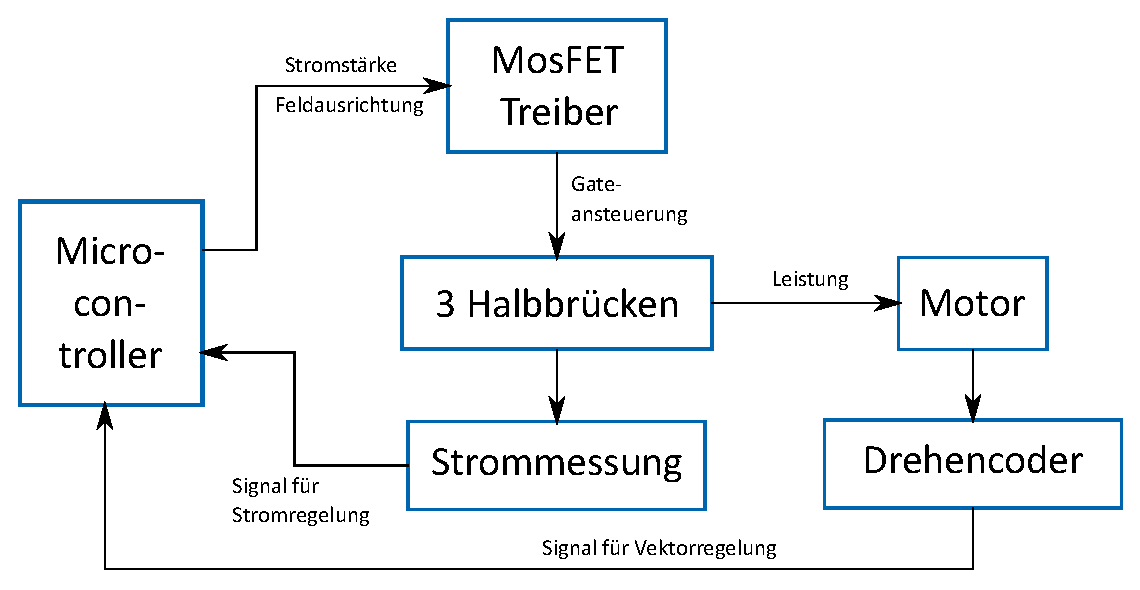
\includegraphics[width=0.8\textwidth]{images/KomponentenVektorregelung.eps}
\caption{notwendige Komponenten eines potentiellen Motortreibers \newline (Quelle: eigene Darstellung, SM)}
\label{kompVec}
\end{figure}

\begin{benannteAuflistung}[Notwendige Komponenten für zwei Motoren:]
    Microcontroller & 12-24 Pwm-Ausgänge pro Motor bei min. 20kHz \\
    & 4-6 digitale Eingänge für Quadraturencoder \\
    & 4 digitale Eingänge für Sollmomentvorgabe (Moment und Richtung) \\
    & 4 analoge Eingänge für Strommessung pro Motor \\
    Leisungstransistoren & 6 Halbbrücken (High-Side-Ansteuerung über Ladepumpe oder Pull-Up Widerstand zur Motorversorgungsspanung)  \\
    Sensorik & 4 mal Strommessung \\
\end{benannteAuflistung}

\par\bigskip

\begin{benannteAuflistung}[Gewünschte Technische Daten:]
    Motorspannung & bis 25V \\
    Strom & dauerhaft 30A, Spitze 50A \\
    Schnittstellen & I2C, USB, PWM \\
\end{benannteAuflistung}

\par\bigskip

Die Herstellungskosten sollten XXX,- € nicht übersteigen.

\par\bigskip



\subsection{Marktanalyse}

\subsubsection{VESC}
\label{sssec:vesc}
Der VESC - vector electronic speed control \cite{vesc} ist ein openSource Projekt von Benjamin Vedder. Der Treiber wurde ausgelegt, um ein Skateboard mit einem bürstenlosen Gleichstrommotor anzutreiben und ist in der Lage, 240A Spitzenstrom und 50A Dauerstrom bei bis zu 60V Versorgungsspannung zu liefern. Er verfügt über eine umfangreiche Konfigurationssoftware, über die vom PC aus alle nötigen Voreinstellungen vorgenommen werden können. Das ganze Projekt wirkt auf den ersten Eindruck sehr ausgereift.


\par\bigskip
\begin{benannteAuflistung}[Technische Daten:]
    Microcontroller & STM34F4 \\
    MOSFET Treiber & DRV8302 \\
    MOSFETS & 6 IRFS7530 \\
    Motorspannung & 8V - 60V \\
    Strom & dauerhaft 50A, Spitze 240A \\
    Schnittstellen & PPM signal (RC servo), analog, UART, I2C, USB, CAN-Bus \\
    Größe & 40mm mal 60mm \\
\end{benannteAuflistung}

\par\bigskip


\begin{benannteAuflistung}[Kosten im Eigenbau für zwei Stück:]
    Bauteile & ca. 120,- € \\
    Platinen & ca. 100,- €\\
    Lötzubehör & ca. 20,- € \\
    \textbf{Summe} & \textbf{ca. 240,- €} \\
\end{benannteAuflistung}

\par\bigskip
Beschaffungskosten für zwei fertig aufgebaute Platinen: \textbf{ca. 280,-€}

\subsubsection{ODrive}
\label{sssec:odrive}
Der ODrive ist eine Entwicklung verschiedener Personen, da grundsätzlich jeder an der Entwicklung des Treibers teilnehmen kann. Dieser Treiber steuert bis zu zwei Motoren mit je ca. 100A Spitzenstrom. Das Projekt befindet sich noch in der Entwicklungsphase. Die Konfiguration des Treibers muss in die Firmware kompiliert werden.

\par\bigskip




\par\bigskip
\newpage
\begin{benannteAuflistung}[Technische Daten:]
    Microcontroller & STM34F4 \\
    MOSFET Treiber & DRV8301 \\
    MOSFETS & 28 NTMFS4935NT1G \\
    Motorspannung & 8V - 30V \\
    Strom & dauerhaft ?, Spitze > 100A \\
    Schnittstellen & USB, CAN, UART, PWM, and step/dir interface \\
    Größe & 110mm mal 50mm \\
\end{benannteAuflistung}


\par\bigskip



\begin{benannteAuflistung}[Kosten im Eigenbau pro Stück:]
    Bauteile & ca. ???,- € \\
    Platinen & ca. ???,- €\\
    Lötzubehör & ca. 20,- € \\
    \textbf{Summe} & \textbf{ca. ???,- €} \\
\end{benannteAuflistung}

\par\bigskip
Beschaffungskosten als fertig aufgebaute Platine: \textbf{ca. 120,-€}

\subsubsection{Predriver}
Zur effizienteren Nutzung der MosFET wird von verschiedenen Herstellern ein Predriver angeboten. Zur Verfügung steht z.B. der DRV8305 von TI. Er stellt als Funktionen die nötige Ladepumpe, eine Möglichkeit zur Strommessung, optimierte Schaltung der FETs und andere Funktionen zur Verfügung.

\subsubsection{fertige Halbbrücke als Smd-Bauteil}
Infineon hat fertige Halbbrücken im Programm, die einige der benötigten Anforderungen bereits ohne externe Komponenten erfüllen. Als Beispiel sei hier der BTN8962TA vorgestellt:

\par\bigskip
\begin{benannteAuflistung}[BTN8962TA]
    Strom & dauerhaft 30A, Spitze 70A \\
    Spannung & bis 40V \\
	Ladepumpe & integriert \\
	Strommessung & integriert \\
	PWM & bis 25kHz \\
	Ansteuerung & logic level \\
	benötigte Menge & 6 Stück \\
	Einzelpreis & ca. 4,22€ \\
	\textbf{Gesamtkosten} & \textbf{ca. 25,-€} \\
\end{benannteAuflistung}

\subsubsection{Aufbau der Halbbrücken aus Einzelkompoenten}
\begin{benannteAuflistung}[Benötigte Komponenten][llX]
    MosFETs & 6 n-FETs  & ca. 3,-€ \\
	& 6 p-FETs & ca. 3,-€ \\
	Predriver & zB & ca. 5,-€ \\
	Strommessung & 4 Shuntwiderstände & ca. 3,-€ \\
	\textbf{Gesamtkosten} & & \textbf{ca. 14,-€} \\
\end{benannteAuflistung}

\subsubsection{Auswahl eines Microcontrollers}
\begin{benannteAuflistung}[Benötigte Eigenschaften pro Motor]
    6 Pwm-Ausgänge pro Motor bei min. 20kHz \\
    6 digitale Ausgänge pro Motor \\
    2-3 digitale Eingänge für Quadraturencoder \\
    2 digitale Eingänge für Sollmomentvorgabe (Moment und Richtung) \\
    2 analoge Eingänge für Strommessung pro Motor \\
\end{benannteAuflistung}
\par\bigskip

Zusätzlich zu den o.g. Angaben muss der Controller gut programmierbar sein und sollte keine, für die Projekt- und Labormitarbeiter völlig neuartige, Programmierumgebung darstellen. Auf Grund dieser Vorgabe wird die Auswahl eingeschränkt auf Controller, die entweder von dem Arduino-Framework oder dem mbed-Framework unterstützt werden.
\par
\begin{benannteAuflistung}[mögliche Kanditaten]
    Atmega 1280 & ca. 9,-€ \\
    Atmega 2560 & ca. 10,-€ \\
    STM32F4 & ca. 9,-€ \\
    STM32F7 & ca. 10,-€ \\
\end{benannteAuflistung}
\par\bigskip
Die Controller von Atmel liegen bei gleichem Preis in ihrer Leistung deutlich unter der Leistung der Controller von ST.

\subsubsection{Komplettlösungen als integrierter Schaltkreis}
Auf dem Markt finden sich verschiedene Ein-Chip-Lösungen für den Betrieb eines Synchronmotors. Jedoch sind diese in der Regel für sensorlosen Antrieb ausgelegt und damit im Stillstand nicht gut betreibbar. Des Weiteren liegen die erreichbaren Ströme weit unter den Projektanforderungen.

\subsection{Fazit}
Der Ankauf fertiger Motortreiber ist zu teuer. Ein eigenständiger Nachbau der Controller Vesc (siehe \ref{sssec:vesc}) oder ODrive (siehe \ref{sssec:odrive}) wird in etwa die gleichen Kosten produzieren, wie die Anschaffung der fertig bestückten Platinen und zusätzliche Arbeit schaffen.
Andere fertige Lösungen stehen derzeit nicht zur Verfügung.\\
 Es erscheint demnach am Sinnvollsten, einen an die Projektanforderungen angepassten Controller im Eigenbau neu zu entwerfen.

% !TEX root = SegwayDoku.tex
\renewcommand{\autoren}{Stephan Morongowski}
\newpage
\section{Navigation}
\subsection{Sensorik}
Zur Verfügung stehen folgende Sensoren:
\begin{itemize}
\item Gyros in allen drei Raumachsen
\item Beschleunigungssensoren in allen drei Raumachsen
\item Inkrementalgeber der Räder
\item Ultraschallsensoren
\end{itemize}

\subsection{Bestimmung der Position im Welt-KS}

\subsubsection{Drehung um den Momentanpol}
\label{turningVelocityPole}
Zur Bestimmung der Position des Roboters in einem festen Koordinatensystem können die Inkrementalgeber der Antriebsmotoren benutzt werden.

\begin{figure}[h]  % [h] bedeutet, dass das Bild genau an dieser Stelle im Text erscheint
\centering\includegraphics[width=0.8\textwidth]{images/Kurvenkinematic.eps}
\caption[Rotation um den Momentanpol]{Rotation um den Momentanpol, hierbei gilt die Annahme, dass die Geschwindigkeiten der Räder während des betrachteten Zeitraumes konstant sind. \newline(Quelle: eigene Darstellung, SM)}
\label{kurvenkinematik}
\end{figure}

Zur Ermittlung der aktuellen Position ist in Abbildung \ref{kurvenkinematik} die Kinematik einer Kurvenfahrt dargestellt, betrachtet für einen gedanklich sehr kleinen Zeitabschnitt. In diesem wird angenommen, dass die Geschwindigkeiten \(v_1\) und \(v_2\) beider Räder konstant bleiben. Dies sorgt für die Vereinfachung, dass der Roboter sich auf einer Kreisbahn um einen für die betrachtete Zeitspanne konstanten Momentanpol bewegt. Im Folgenden sind die durch den Inkrementalgeber erfassten Bogenlängen mit $x_l$  und $x_r$ bezeichnet.
Es gilt:
\begin{flalign}
    % durch das & Zeichen werden alle Gleichungen an diesem Punkt ausgerichtet
	x_l &  = \Delta\gamma\cdot r_l
	\label{eq:bogenmaß_1} \\
	x_r & = \Delta\gamma\cdot r_r
	\label{eq:bogenmaß_2} \\
	r_r & = r_l  + l_a
	\label{eq:achsZuMomentanpol} \\
	\Delta x_{rl} & = x_r - x_l
	\label{eq:arcsDef} \\
    r_S & = r_r - \frac{1}{2} l_a
	\label{eq:r_s}
\end{flalign}

Aus \eqref{eq:bogenmaß_1}, \eqref{eq:bogenmaß_2}, \eqref{eq:achsZuMomentanpol}, \eqref{eq:arcsDef} und \eqref{eq:r_s} folgen:
% hier keine Leerzeile machen, sonst wird der Abstand ganz groß
\begin{flalign}
    \Delta\gamma & = \frac{\Delta x_{rl}}{l_a}
	\label{eq:deltaGamma}	 \\
    r_S & = \frac{x_r}{\Delta\gamma} - \frac{1}{2} l_a =
    l_a\left(\frac{x_r}{\Delta x_{rl}}-\frac{1}{2}\right)
\end{flalign}
Alternative nach Timo Veit:
\begin{flalign}
	x_S &= \frac{x_2-x_1}{2}+x_1	\\
	r_S &=  \frac{l_a}{ \frac{x_2}{x_1}-1} +  \frac{l_a}{2} = 0.5l_a \frac{x_l+x_r}{x_l-x_r}\\
	\Delta\gamma &= atan( \frac{x_S}{r_S})
\end{flalign}
Ende der Alternative \\\\

Durch Aufsummieren von \(\Delta\gamma\) nach jeder Auswertung der Inkrementalgeber kann somit ein ungefährer Absolutwinkel der Roboterachse zu einem festen KS berechnet werden.
\par\bigskip
Zur Bestimmung des Schwerpunktes in xy-Koordinaten wird die Verschiebung von
\(S_0\) zu \(S_1\) mit trigonometrischen Funktionen berechnet und anschließend aufsummiert. Es gilt:
\begin{flalign}
	\vec{S_1} = \vec{S_0} +
        \begin{pmatrix}
            -\sin{(\Delta \gamma)} \cdot r_S \cdot \sin{(\gamma_0)}
            - (r_S - \cos{(\Delta \gamma)} \cdot r_S) \cdot \cos{(\gamma_0}) \\
            \sin{(\Delta \gamma)} \cdot r_S \cdot \cos{(\gamma_0)}
            - (r_S - \cos{(\Delta \gamma)} \cdot r_S) \cdot \sin{(\gamma_0})
        \end{pmatrix}
	\label{eq:S_1}
\end{flalign}

bzw. vereinfacht:
\begin{flalign}
	\vec{S_1} = \vec{S_0} +
        \begin{pmatrix}
            r_S [\cos{(\gamma_0 + \Delta\gamma)} - \cos{\gamma_0}]  \\
            r_S [\sin{(\gamma_0 + \Delta\gamma)} - \sin{\gamma_0}]
        \end{pmatrix}
	\label{eq:S_1_easy}
\end{flalign}

\subsubsection{Algorithmus zur Verwendung in Interrupt-Service-Routinen (ISR)}
\label{easyDeadReckoning}
Nachteilig an der in \ref{turningVelocityPole} beschriebenen Methode sind folgende zwei Punkte: Zum Einen muss eine Geradeausfahrt des Roboters als Spezialfall behandelt werden, da sonst eine Division durch Null erfolgen würde. Zum Zweiten finden die Berechnungen immer nahe einer Singularität statt. Für eine annähernde Geradeausfahrt wird $r_S$ sehr groß und $\Delta \gamma$ sehr klein, was zu großen Berechnungsfehlern führen kann.

Reagiert man nun auf jedes Pulssignal der Inkrementalgeber, wird eine der beiden Größen $x_n$ zu Null und der Momentanpol liegt auf dem Rad, welches sich annähernd nicht bewegt hat. So müssen nur vier Fälle bei der Summation der Lageänderungen beachtet werden:

\begin{itemize}
\item $R_l$ dreht sich vorwärts oder rückwärts
\item $R_r$ dreht sich vorwärts oder rückwärts
\end{itemize}

Für jeden dieser Fälle können nun die Positionsänderungen $\Delta\gamma$, $\prescript{1}{}{\Delta x}$, $\prescript{1}{}{\Delta y}$ im roboterfesten KS vorberechnet werden.
\begin{flalign}
    x_n & = \frac{2\pi\cdot r_R}{n_{Enc}}  \\
	\Delta\gamma & = \frac{x_n}{l_a}  \\
	\prescript{1}{}{\Delta x} & = \frac{1}{2}l_a\sin{(\Delta\gamma)}  \\
	\prescript{1}{}{\Delta y} & = \frac{1}{2}l_a ( \cos{(\Delta\gamma)} - 1) 
\end{flalign}
mit der Weglänge zwischen zwei Encoderimpulsen $x_n$,  \\
der Anzahl der Encoderimpulse pro Umdrehung $n_{Enc}$  \\ 
und dem Radius der Räder $r_R$. \\ \\
Bei jedem Impuls der Encoder werden nun in Abhängigkeit von $\gamma_0$ die vorberechneten Positionsänderungen mit Hilfe einer Drehmatrix in das Welt-KS transformiert und zu $S_0$ hinzuaddiert. Zu $\gamma_0$ wird jedes Mal der konstante Wert $\Delta\gamma$ addiert.
\begin{flalign}
    \prescript{0}{}{S_1} &= \prescript{0}{}{S_0} + \prescript{0}{}{T}_1  \prescript{1}{}{\vec{\Delta s}}
    = \prescript{0}{}{S_0} + 
        \begin{pmatrix}
            \cos{\gamma_0} & -\sin{\gamma_0}  \\
            \sin{\gamma_0} & \cos{\gamma_0}
        \end{pmatrix}
        \begin{pmatrix}
            \prescript{1}{}{\Delta y}  \\
            \prescript{1}{}{\Delta y}  
        \end{pmatrix}
        \label{eq:transformation} \\
    \gamma_1 &= \gamma_0 + \Delta\gamma
\end{flalign}
Nachteilig ist hier insbesondere bei hohen Fahrtgeschwindigkeiten des Roboters eine starke Prozessorauslastung.
\subsubsection{Berücksichtigung des Kippwinkels}
\label{duKipper}
Obiger Algorithmus setzt voraus, dass der Roboter aufrecht steht. Kippt der Roboter um seine y-Achse, werden alleine durch das Kippen die Encoder verdreht, was zu einer berechneten Positionsänderung führt, die gar nicht stattgefunden hat. Um dies zu kompensieren, reichen die Encoder als alleinige Information nicht aus. Da der Roboter einen Sensor zur Bestimmung des Kippwinkels besitzt, kann nun eine laufende Korrektur vorgenommen werden. Dabei ist zu beachten, dass der Fehler durch das Kippen auch von dem aktuellen Winkel $\gamma$ abhängig ist. Kippt der Roboter z.B. bei einem $\gamma$ von $0°$, entsteht ein Fehler in x-Richtung. Würde er sich nun auf der Stelle drehen auf ein $\gamma$ von $90\degree$ und der bei einem $\gamma$ von $0\degree$ entstandene Fehler weiterhin einfach abgezogen, würde die Position nun einen Ort mit einem Fehler in y-Richtung anzeigen. Deshalb wird bei jedem Encoderimpuls die Änderung des Kippwinkels im Vergleich zur letzten Encoderauswertung umgerechnet in einen Weg in x-Richtung des roboterfesten KS, anschließend in das Welt-KS transformiert und gleichzeitig mit der durch in Abschnitt \ref{easyDeadReckoning} falsch berechneten Welt-Position aufsummiert. Problematisch ist hier ein Kippen des Roboters, bei dem die Räder sich mit ebenfalls mit der gleichen Winkelgeschwindigkeit des Roboterkörpers drehen. In diesem Fall werden keine Encoderimpulse erzeugt und die Berechnung der Position nicht durchgeführt, was kurzzeitig zu falschen Angaben und Sprüngen in der Position führen kann.

\subsubsection{Reduktion des Berechnungsaufwandes}
Um eine deutlich geringere Prozessorbelastung zu erreichen, kann die Position z.B. nur nach bestimmten Zeitintervallen oder nach einer bestimmten Anzahl Encoderimpulse aktualisiert werden. Dafür ist eine weitere Anpassung des Algorithmus nötig. Dabei wird die Änderung des Winkels $\Delta\gamma$ nach Gleichung \ref{eq:deltaGamma}	durchgeführt, und die Lageänderung im roboterfesten KS durch 
\begin{flalign}
    \prescript{0}{}{\Delta x_0} & = \frac{x_r-x_l}{2} \\
    \prescript{0}{}{\Delta y_0} & \approx 0
{}\end{flalign}
angenähert und anschließend mit Hilfe Gleichung \ref{eq:transformation} aufsummiert. Möglich wäre auch eine getrennte Auswertung der Encodersignale und der Winkelkorrektur, wobei z.B. nur jeder zehnte Encoderimpuls eine Neuberechnung auslöst und die Winkelkorrektur unabhängig von den Impulsen in festen Zeitabständen berechnet wird. Letzteres würde dazu dienen, das in \ref{duKipper} beschriebene Problem des gleichschnellen Drehens der Räder und des Roboterkörpers zu lösen.

\newpage

% !TEX root = SegwayDoku.tex
\renewcommand{\autoren}{Timo Veit}
\newpage
\section{Auslegung Kurvengeschwindigkeit}

\begin{figure}[h]  % [h] bedeutet, dass das Bild genau an dieser Stelle im Text erscheint
\centering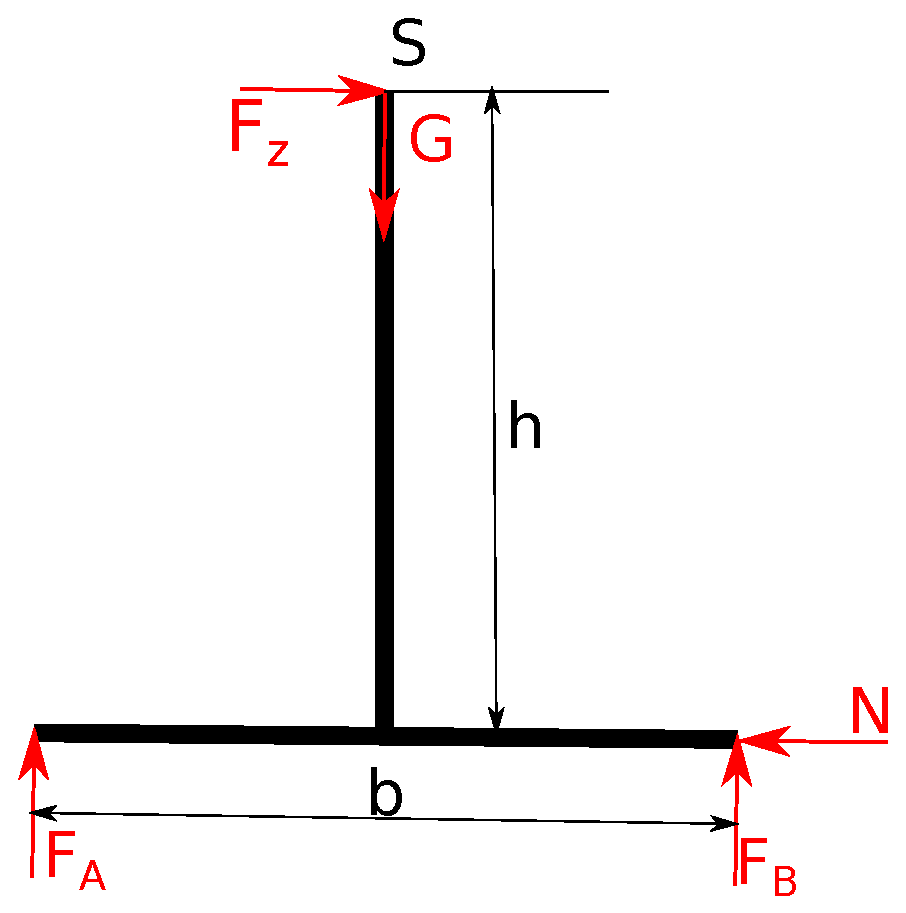
\includegraphics[width=0.6\textwidth]{images/SegwayFliehkraft.eps}
\caption{Kräfte bei der Kurvenfahrt \newline (Quelle: eigene Darstellung, TV)}
\label{zentripetal}
\end{figure}

Bei der Kurvenfahrt darf der Roboter nicht seitlich umkippen. Um dies zu gewährleisten, muss das Verhältnis zwischen Geschwindigkeit und Kurvenradius passen. Dazu soll der innere Reifen noch mindestens die Hälfte der Last aufnehmen wie im Stand also ein Viertel der Gewichtskraft.

Es gilt:
\begin{flalign}
    % durch das & Zeichen werden alle Gleichungen an diesem Punkt ausgerichtet
	F_A &  = \frac{1}{4} m \cdot g
	\label{eq:gewichtskraft_1} \\
	G &  = m \cdot g
	\label{eq:gewichtskraft_2} \\
	F_{z} & = m \cdot \ddot x
	\label{eq:zentrifugalkraft} \\
	N & = m \cdot \frac{v^{2}}{r}
	\label{eq:zentripetalkraft} \\
	F_{A} + F_{B} & = G
	\label{eq:vertikale} \\
	N & = F_{z}
	\label{eq:horizontale} \\
    F_A \cdot b & = F_z \cdot h
	\label{eq:moment}
\end{flalign}

Hieraus folgt:
% hier keine Leerzeile machen, sonst wird der Abstand ganz groß
\begin{flalign}
    \ddot x & = \frac{v^{2}}{r}
	\label{eq:xpp} \\
    \frac{1}{4} m \cdot g \cdot b & = m \cdot \frac{v^{2}}{r} \cdot h
	\label{eq:lsg_1}
\end{flalign}

Und daraus die Zusammenhänge von Geschwindigkeit zu Radius
\begin{flalign}
    v & = \sqrt{\dfrac{gb}{4h} \cdot r}
	\label{eq:lsg_v} \\
    r & = \dfrac{4h}{gb} \cdot v^2
	\label{eq:lsg_r}
\end{flalign}

Der notwendige Reibwert \(\mu\) zwischen Reifen und Boden ergibt sich aus der Haftbedingung.

\begin{flalign}
    \mu \cdot mg & = m \cdot \frac{v^{2}}{r}
	\label{eq:mu_1} \\
    \mu & = \frac{v^{2}}{rg}
	\label{eq:mu_2}
\end{flalign}

Mit diesen Werten könnte man die Kurvengeschwindigkeit des Roboters begrenzen.

\newpage

